
\documentclass[12pt]{article}
\usepackage{pgf}
\usepackage{pgflibraryshapes}
\usepackage{tikz}

\begin{document}

\thispagestyle{empty}
\setlength{\fboxrule}{0.01pt}
\setlength{\fboxsep}{4pt}

\fbox{

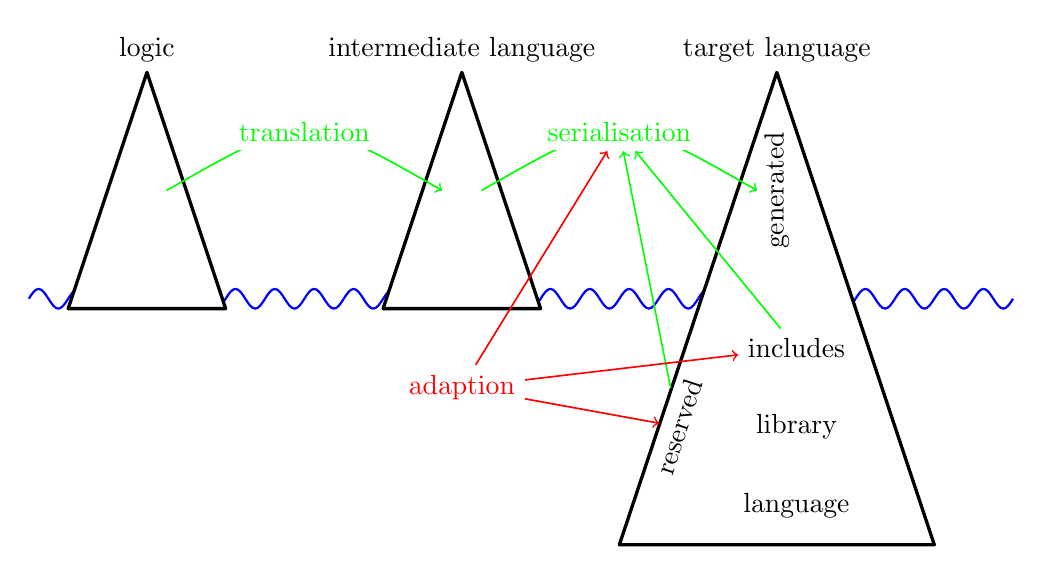
\begin{tikzpicture}[scale = 0.5]
  \tikzstyle water=[color = blue, thick]
  \tikzstyle ice=[color = black, very thick, cap = round, join = round, fill = white]
  \tikzstyle process=[color = green, semithick, ->]
  \tikzstyle adaption=[color = red, semithick, ->]
  \tikzstyle target=[color = black]
  \foreach \x in {0, ..., 24}
    \draw[style=water] (\x, 0.25) sin + (0.25, 0.25) cos + (0.25, -0.25) sin
      + (0.25, -0.25) cos + (0.25, 0.25);
  \draw[style=ice] (1, 0) --
    (3, 6) node[above, fill=white] {logic} -- (5, 0) -- cycle;
  \draw[style=ice] (9, 0) --
    (11, 6) node[above, fill=white] {intermediate language} -- (13, 0) -- cycle;
  \draw[style=ice] (15, -6) --
    (19, 6) node[above, fill=white] {target language} -- (23, -6) -- cycle;
  \draw[style=process]
    (3.5, 3) .. controls (7, 5) .. node[fill=white] {translation} (10.5, 3);
  \draw[style=process]
    (11.5, 3) .. controls (15, 5) .. node[fill=white] (serialisation) {serialisation} (18.5, 3);
  \node (adaption) at (11, -2) [style=adaption] {adaption};
  \node at (19, 3) [rotate=90] {generated};
  \node at (19.5, -5) {language};
  \node at (19.5, -3) {library};
  \node (includes) at (19.5, -1) {includes};
  \node (reserved) at (16.5, -3) [rotate=72] {reserved}; % proper 71.57
  \draw[style=process]
    (includes) -- (serialisation);
  \draw[style=process]
    (reserved) -- (serialisation);
  \draw[style=adaption]
    (adaption) -- (serialisation);
  \draw[style=adaption]
    (adaption) -- (includes);
  \draw[style=adaption]
    (adaption) -- (reserved);
\end{tikzpicture}

}

\end{document}
